\documentclass{article}

\usepackage{fancyhdr}
\usepackage{extramarks}
\usepackage{amsmath}
\usepackage{amsthm}
\usepackage{amsfonts}
\usepackage{tikz}
\usepackage[plain]{algorithm}
\usepackage{algpseudocode}

\usetikzlibrary{automata,positioning}

\usepackage{graphicx}
\graphicspath{ {./images/} }

%
% Basic Document Settings
%

\topmargin=-0.45in
\evensidemargin=0in
\oddsidemargin=0in
\textwidth=6.5in
\textheight=9.0in
\headsep=0.25in

\linespread{1.1}

\pagestyle{fancy}
\lhead{Yousef Alaa Awad}
\chead{\hmwkClass\: \hmwkTitle}
\rhead{\firstxmark}
\lfoot{\lastxmark}
\cfoot{\thepage}

\renewcommand\headrulewidth{0.4pt}
\renewcommand\footrulewidth{0.4pt}

\setlength\parindent{0pt}

%
% Create Problem Sections
%

\setcounter{secnumdepth}{0}
\newcounter{partCounter}
\newcounter{homeworkProblemCounter}
\setcounter{homeworkProblemCounter}{1}

\newcommand{\hmwkTitle}{Homework\ \#2}
\newcommand{\hmwkDueDate}{September 5, 2025}
\newcommand{\hmwkClass}{Power Systems Economics}

%
% Title Page
%

\title{
    \vspace{2in}
    \textmd{\textbf{\hmwkClass:\ \hmwkTitle}}\\
    \normalsize\vspace{0.1in}
    \vspace{3in}
}

\author{Yousef Alaa Awad}

% Problems start here
\begin{document}

\maketitle
\pagebreak

\section{2.5}
\textbf{Given:}  The demand curve for a product is estimated to be given by the expression: $$ q = 200 - \pi $$

\subsection{A) Calculate the price and the price elasticity of the demand for the following values of the demand.}
First, in general we have to find the derivative of the demand related to the price $\pi$.
$$ \frac{\text{d}q}{\text{d}\pi} = -1$$

\subsubsection{i) q = 0}
Now, specifically when the demand, q, is 0 (and the same for the following calculations for the rest of this subsection), we simply need to find out the price, $\pi$ that the amount consumed would be sold at.
$$ 0 = 200 - \pi \rightarrow -200 = -\pi \rightarrow \pi = 200 $$

Now, to calculate the price elasticity we use the following general equation:
$$ \frac{\text{d}q}{\text{d}\pi}*\frac{\pi}{q} $$
And when plugged into the equation we do the following algebra:
$$ \frac{\text{d}q}{\text{d}\pi}*\frac{\pi}{q} = (-1)*\frac{200}{0} $$
BUT, UH OH, we have a problem in that we cannot divide by 0/this specific demand value. To solve this we simply use an approximation using the limit definition of $q=0$, and therefore we \textit{actually} have the following equation:
$$ (-1)*\frac{200}{\lim_{x \to 0} q} \rightarrow (-1)*\frac{200}{0.000...001} \rightarrow (-1)*(\infty) \rightarrow \varepsilon = -\infty $$
Now, what in the world is the meaning of this. What does a price elasticity of $-\infty$ even mean? Well, it means that the consumers/demanders are \textit{extremely} sensitive to price changes, and therefore the elasticity of demand is \textbf{perfectly elastic demand}.

\subsubsection{ii) q = 50}
Now, for a $q=50$, we really do the same method of calculation as the last (and therefore there will be alot less explaining from now on). Where first we calculate the price, $\pi$, then simply plug it in.
$$ q = 200 - \pi \rightarrow 50 = 200 - \pi \rightarrow -150 = -\pi \rightarrow \pi = 150 $$
And now we plug it in.
$$ \frac{\text{d}q}{\text{d}\pi}*\frac{\pi}{q} \rightarrow (-1)*\frac{150}{50} \rightarrow (-1)*(3) \rightarrow \varepsilon = -3 $$
And, to interpret this $\varepsilon = -3$, it simply means that we have an \textbf{elastic price elasticity} where a 1\% increase in price leads to a 3\% decrease (due to $\frac{\text{d}q}{\text{d}\pi}$ being a negative number) in demand.

\subsubsection{iii) q = 100}
And now, less words...
$$ q = 200 - \pi \rightarrow 100 = 200 - \pi \rightarrow -100 = -\pi \rightarrow \pi = 100 $$
And when plugged into the price elasticity equation we get:
$$ \frac{\text{d}q}{\text{d}\pi}*\frac{\pi}{q} \rightarrow (-1)*\frac{100}{100} \rightarrow (-1)*1 \rightarrow \varepsilon = -1 $$
This price elasticity of demand specifically means we have the mythical \textbf{unit elastic demand} where a 1\% increase in price creates a 1\% decrease in price.

\subsubsection{iv) q = 150}
$$ q = 200 - \pi \rightarrow 150 = 200 - \pi \rightarrow -50 = -\pi \rightarrow \pi = 50 $$
And when plugged into the price elasticity equation we get:
$$ \frac{\text{d}q}{\text{d}\pi}*\frac{\pi}{q} \rightarrow (-1)*\frac{50}{150} \rightarrow (-1)*\frac{1}{3} \rightarrow \varepsilon = -\frac{1}{3} $$
This price elasticity of demand specifically means we have \textbf{inelastic demand} where a 1\% increase in price creates a $\frac{1}{3}$\% decrease in price.

\subsubsection{v) q = 200}
$$ q = 200 - \pi \rightarrow 200 = 200 - \pi \rightarrow 0 = -\pi \rightarrow \pi = 0 $$
And when plugged into the price elasticity equation we get:
$$ \frac{\text{d}q}{\text{d}\pi}*\frac{\pi}{q} \rightarrow (-1)*\frac{0}{200} \rightarrow (-1)*0 \rightarrow \varepsilon = 0 $$
This price elasticity of demand specifically means we have the mythical \textbf{perfectly inelastic demand} where a 1\% increase in price creates \textbf{no} decrease in price.
\pagebreak

\subsection{B) Repeat the calculations for the case in which the demand curve is given by the expression: $$ q = \frac{10,000}{\pi} $$}
Now, just like above we must first calculate the derivative of the demand, q, in relation to the price, $\pi$.
$$ \frac{\text{d}q}{\text{d}\pi} = -\frac{10,000}{\pi^2}$$

And remember that the equation for price is just the algebraic conversion of the following:
$$ q = \frac{10,000}{\pi} \rightarrow q*\pi = 10,000 \rightarrow \pi = \frac{10,000}{q} $$
And note that the equation for elasticity is simply...
$$ \varepsilon = \frac{\text{d}q}{\text{d}\pi}*\frac{\pi}{q} $$

And so, I will simply be plugging in the values to the following demand values...

\subsubsection{i) q = 0}
$$ \pi = \frac{10,000}{q} = \frac{10,000}{0} \approx \infty $$

$$ \varepsilon = \frac{\text{d}q}{\text{d}\pi}*\frac{\pi}{q} = -\frac{10,000}{\infty^2}*\frac{\infty}{0} = -1*\frac{\infty^2}{\infty^2} = -1$$

\subsubsection{ii) q = 50}
$$ \pi = \frac{10,000}{q} = \frac{10,000}{50} = \$200 $$

$$ \varepsilon = \frac{\text{d}q}{\text{d}\pi}*\frac{\pi}{q} = -\frac{10,000}{\pi^2}*\frac{\pi}{q} = -\frac{10,000}{200^2}*\frac{200}{50} = -1 $$

\subsubsection{iii) q = 100}
$$ \pi = \frac{10,000}{q} = \frac{10,000}{100} = \$100 $$

$$ \varepsilon = \frac{\text{d}q}{\text{d}\pi}*\frac{\pi}{q} =  -\frac{10,000}{\pi^2}*\frac{\pi}{q} = -\frac{10,000}{100^2}*\frac{100}{100} = -1$$

\subsubsection{iv) q = 150}
$$ \pi = \frac{10,000}{q} = \frac{10,000}{150} = \$66.67 $$

$$ \varepsilon = \frac{\text{d}q}{\text{d}\pi}*\frac{\pi}{q} = -\frac{10,000}{\pi^2}*\frac{\pi}{q} = -\frac{10,000}{66.67^2}*\frac{66.67}{150} = -1 $$

\subsubsection{v) q = 200}
$$ \pi = \frac{10,000}{q} = \frac{10,000}{200} = \$50 $$

$$ \varepsilon = \frac{\text{d}q}{\text{d}\pi}*\frac{\pi}{q} = -\frac{10,000}{\pi^2}*\frac{\pi}{q} = -\frac{10,000}{50^2}*\frac{50}{200} = -1 $$

\subsection{Python Script Output Verification}
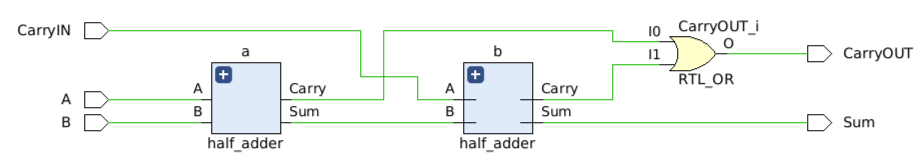
\includegraphics[width=\textwidth]{apple.png}

\pagebreak
\section{2.8}
\textbf{Given:} A firm's short-run cost function for the production of gizmos is given by the following expression: $$ C(y) = 10*y^2 + 200*y + 100,000 $$

\subsection{A) Calculate the range of output over which it would be profitable for this firm to produce gizmos if it can ell each gizmo for \$2400. Calculate the value of the output that maximizes this profit.}
The profitable range is when the price is larger than the average  cost, $\text{AC}(y)$, is defined as the following:
$$ \text{AC}(y) = \frac{\text{C}(y)}{y} = \frac{10*y^2 + 200*y + 100,000}{y} = 10*y + 200 + \frac{100,000}{y}$$
And therefore the range is....
$$ 2400 > 10*y + 200 + \frac{100,000}{y} \rightarrow 2200 > 10*y + \frac{100,000}{y} \rightarrow 0 > 10*y + \frac{100,000}{y} - 2200 $$
$$ \rightarrow 0 > 10*y^2 - 2200*y + 100,000 $$
And when you find the roots/zeros of this function you get the a minimum of 65 and a maximum of 155, meaning the range of output is \textbf{65 $\le$ y $\le$ 155}. \newline
Now the value that maximizes the profits would be when the Marginal Cost (MC) and Marginal Revenue (MR) are equivalent. In this case, the Marginal Revenue was given to us at a value of \$2400. The Marginal Costs, however, we have to calculate:
$$ \text{MC} = \frac{\text{d}C}{\text{d}y} = 20*y + 200$$
$$ \text{MC} = \text{MR} \rightarrow 2400 = 20*y + 200 \rightarrow 2200 = 20*y \rightarrow y = 110$$
Therefore, we know that the profit is maximized at an output of \textbf{110 gizmos} at a price of \$2400.

\subsection{B) Repeat these calculations and explain your results for the case in which the short-run cost function is given by $$ C(y) = 10*y^2 + 200*y + 200,000 $$}
Since we have a new Cost function we must first verify that the Marginal Cost is also the same (as then the profit maximization point is also the same):
$$ \frac{\text{d}C}{\text{d}y} = 20*y + 200 $$
Thankfully, in this case it is the same. After this we then need to find the profit function.
$$ \Pi(y) = R - C = 2400*y - (10*y^2 + 200*y + 200,000)  = -10*y^2 + 2200*y - 200,000$$
And since the optimal output at that price is also the same as above (aka 110 Gizmos), we find that the maximum possible profit is the following:
$$ \Pi(110) = -10*(110)^2 + 200*(110) - 200,000 = -\$79,000 $$
This maximum profit, is sadly negative though. Meaning that the fixed costs (the \$200,000 constant in the Cost equation) are too high to sustain any profits at any production level.

\end{document}
